% !Mode:: "TeX:UTF-8"
% !TEX program  = xelatex

\documentclass{cumcmthesis}
%\documentclass[withoutpreface,bwprint]{cumcmthesis} %去掉封面与编号页
%\usepackage{ctex}    
%用了第一行的documentclass里已经包含了大部分数学公式需要的宏包,不需要再引入了


\title{高压油管的压力控制模型研究}
\tihao{A}
\baominghao{201919029020}
\schoolname{南方科技大学}
\membera{熊卓晨}
\memberb{邓钧泽}
\memberc{孔祥喆}
\supervisor{李景治老师}
\yearinput{2019}
\monthinput{09}
\dayinput{12}

\begin{document}
\maketitle

 
 \begin{abstract}
 	摘要的具体内容,我也不知道下写点啥,先占个座吧。
 	\keywords{关键词1\quad  关键词2\quad   关键词3}
 \end{abstract}

%目录
\tableofcontents

\newpage
\section{问题背景}
燃油进入和喷出高压油管是许多燃油发动机工作的基础,\cref{fig:youtube-picture} 给出了某高压
燃油系统的工作原理,燃油经过高压油泵从 A 处进入高压油管,再由喷口 B 喷
出。燃油进入和喷出的间歇性工作过程会导致高压油管内压力的变化,使得所喷
出的燃油量出现偏差,从而影响发动机的工作效率。

\begin{figure}[!h]
	\centering %图片全局居中
	%并排几个图,就要写几个minipage
	\begin{minipage}[b]{0.4\textwidth} %所有minipage宽度之和要小于1,否则会自动变成竖排
		\centering %图片局部居中
		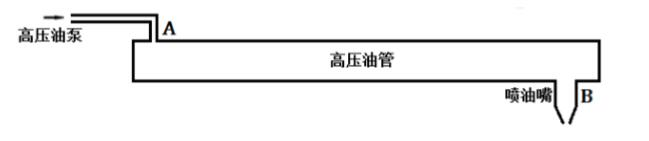
\includegraphics[width=1\textwidth]{youtube} %此时的图片宽度比例是相对于这个minipage的,不是全局
		\caption{高压油管示意图}
		\label{fig:youtube-picture}
	\end{minipage}
	\begin{minipage}[b]{0.4\textwidth} %所有minipage宽度之和要小于1,否则会自动变成竖排
		\centering %图片局部居中
		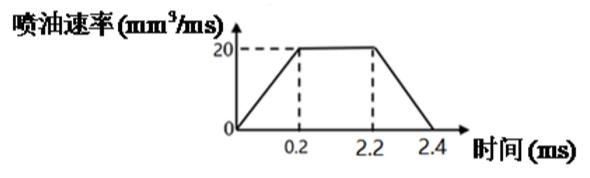
\includegraphics[width=1\textwidth]{penyousudu}%此时的图片宽度比例是相对于这个minipage的,不是全局
		\caption{喷油速率示意图}
		\label{fig:penyou-picture}
	\end{minipage}
\end{figure}
题目中某个高压油管的基本参数如下:

高压油管的内腔长度为 500mm,内直径为 10mm,供油入口
A 处小孔的直径为 1.4mm,通过单向阀开关控制供油时间的长短,单向阀每打开
一次后就要关闭 10ms。喷油器每秒工作 10 次,每次工作时喷油时间为 2.4ms,
喷油器工作时从喷油嘴 B 处向外喷油的速率如 \cref{fig:penyou-picture} 所示。高压油泵在入口 A 处提供的压力恒为 160 MPa,高压油管内的初始压力为 100 MPa。
\section{问题的提出}
\subsection{问题重述}
由题目给出的背景知识及三个问题可以分析出本文共需解决n个问题,通过解决这n个问题建立模型分析在高压油管中多个不同参数改变的情况下,如何调整油泵参数使发动机工作效率最大化。这些问题分别为:

\begin{enumerate}
	\item 要将高压油管内的压力尽可能稳定在 100 MPa 左右,如何设置单向阀每次开启的时长?
	\item 要将高压油管内的压力从 100 MPa 增加到 150 MPa,且分别经过约 2 s、5 s 和10 s 的调整过程后稳定在 150 MPa,单向阀开启的时长应如何调整? 
	\begin{figure}[!h]
		\centering %图片全局居中
		%并排几个图,就要写几个minipage
		\begin{minipage}[b]{0.6\textwidth} %所有minipage宽度之和要小于1,否则会自动变成竖排
			\centering %图片局部居中
			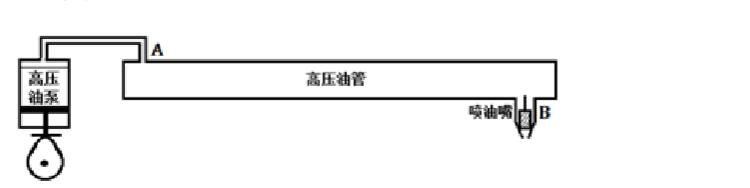
\includegraphics[width=1\textwidth]{realyoutube} %此时的图片宽度比例是相对于这个minipage的,不是全局
			\caption{高压油管实际工作示意图}
			\label{fig:realyoutube-picture}
		\end{minipage}
		\begin{minipage}[b]{0.39\textwidth} %所有minipage宽度之和要小于1,否则会自动变成竖排
			\centering %图片局部居中
			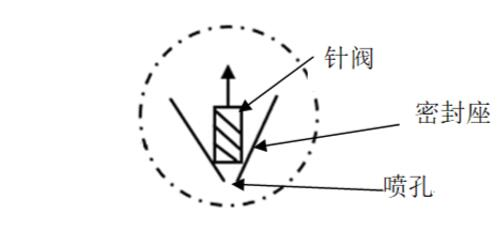
\includegraphics[width=1\textwidth]{muzzle}%此时的图片宽度比例是相对于这个minipage的,不是全局
			\caption{喷油器喷嘴示意图 }
			\label{fig:muzzle-picture}
		\end{minipage}
	\end{figure}
	\item 实际工作中,高压油管A处的燃油来自高压油泵的柱塞腔出口,喷油由喷油嘴的
	针阀控制。高压油泵柱塞的压油过程如\cref{fig:realyoutube-picture}所示,
	凸轮驱动柱塞上下运动。针阀的结构如\cref{fig:muzzle-picture}所示,
	燃油通过针阀的开闭喷出。在题目给出的基本参数条件下,
	确定凸轮的角速度,使得高压油管内的压力尽量稳定在100 MPa左右。
	
	\item 在上一问的基础上,再增加一个喷油嘴,每个喷嘴喷油规律相同,喷
	油和供油策略应如何调整?
	\begin{figure}[!h]
			\centering %图片局部居中
			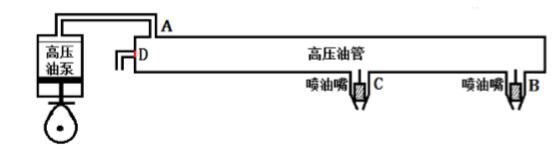
\includegraphics[width=0.8\textwidth]{doublemuzzle}
			\caption{具有减压阀和两个喷油嘴时高压油管示意图 }
			\label{fig:doublemuzzle-picture}
	\end{figure}

	\item 为了更有效地控制高压油管的压力,现计划在D处安
	装一个单向减压阀(\cref{fig:doublemuzzle-picture})。单向减压阀出口为直径为1.4mm的圆,打开后高压油
	管内的燃油可以在压力下回流到外部低压油路中,从而使得高压油管内燃油的压
	力减小。请给出高压油泵和减压阀的控制方案。 
\end{enumerate}
\subsection{问题分析}
\begin{enumerate}
	\item 根据题意,要尽可能维持高压油管内的压力为100Mpa,则单向阀闷的入油质量和喷油嘴的出油质量应尽量维持在相等状态。由给出的公式可以求出不同压强条件下的燃油密度,再根据入油和出油的体积,建立方程式,解出维持100Mpa所需要的单向阀每次开启的时间。
	\item 如果要将燃油压强提升到150Mpa,其实质是高压油管中燃油质量的增加,先计算出燃油质量的增量,再建立相应方程式,解出单向阀每次开启的时间。其中,由于高压油管内的压强再时刻变化,需要做相应的近似处理。
	\item
	\item
	\item
\end{enumerate}
\section{模型基本假设}
\section{符号说明}
\begin{center}
	\begin{tabular}{cc}
		\toprule
		\makebox[0.3\textwidth][c]{符号}	&  \makebox[0.4\textwidth][c]{意义} \\ \midrule
		D	    & 木条宽度(cm) \\ 
		F       & 测试用例(cm)\\
		\bottomrule
	\end{tabular}
\end{center}
\section{模型的构建与求解}

\section{总结}
\subsection{模型的评价}
\subsubsection{模型的优点}
\subsubsection{模型的缺点}
\subsection{模型的改进}
\subsection{模型的推广}

%参考文献
\begin{thebibliography}{9}%宽度9
	\bibitem{bib:one}
\end{thebibliography}

\begin{appendices}
	附录的内容。
\end{appendices}


\end{document}
